
\setcounter{chapter}{0}
\chapter{La probabilit\`{a} e la distribuzione di probabilit\`{a}} 

\section{Assiomi di Kolgomorov}
\textcolor{blue}{Come si definisce la probabilit\'{a} secondo Kolgomorov?}\newline

Consideriamo degli eventi $E_1,E_2 \subset \Omega$ spazio campione, vogliamo costruire definiamo probabilit\'{a} una un funzione $P: \Omega \rightarrow [0,1] $ che soddisfa le seguenti propriet\'{a}:

\begin{itemize}
	\item $P(\Omega) = 1$
	\item $\forall A \subset \Omega$ si ha che $P(A) \geq 0$
	\item $\forall A,B \subset \Omega$,  si ha che $P(A \cup B) = P(A) + P(B) - P(A \cap B)$. Se gli eventi sono indipendenti $ A \cap B = \varnothing $, si ha che $P(A \cup B) = P(A) + P(B)$. 
\end{itemize}

 
\subsection{Definizione di probabilit\'{a} frequentista}

\textcolor{blue}{Come si definisce operativamente la probabilit\'{a} secondo la formulazione frequentista?}\newline

La probabilit\'{a} di un evento A \'{e} definita come il rapporto tra il numero di casi favorevoli (in cui avviene l'evento A) e il numero di casi possibili ( la popolazione). Consideriamo di avere \textbf{N} eventi, e di contare il numero di volte in cui l'evento A, indicandolo come \textbf{n(A)}. Definiamo la probabilit\'{a} di un evento come:
\begin{equation}
	\lim_{N \rightarrow \infty } \dfrac{n(A)}{N}
\end{equation} 

\noindent dove il limite \'{e} inteso in senso probabilistico ovvero al crescere del numero degli eventi.
\subsubsection{Probabilit\'{a} condizionata}

\textcolor{blue}{Che cos'\'{e} la probabilit\'{a} condizionata ?} \newline

Consideriamo una coppia di eventi $A,B \subset \Omega$ definiamo \textbf{probabilit\'{a} condizionata} la probabilit\'{a} che si verifichi l'evento A al verificarsi previamente dell'evento B. 

\begin{equation}
	P(A \vert B) = \dfrac{P(A\cap B)}{P(B)}
\end{equation}

\noindent si dimostra che la probabilit\'{a} condizionata soddisfa gli assiomi di Kolgomorov.

\noindent Nel caso di due eventi indipendenti, ovvero che il verificarsi di B non influenza la probabilit\'{a} che si verifichi A

\begin{equation*}
	P(A \vert B) = P(A \vert \Omega) = P(A)
\end{equation*}

\noindent per due eventi indipendenti possiamo riscrivere la probabilit\'{a} condizionata come:

\begin{equation}
	P(A \cap B) = P(A) \cdot P(B)
\end{equation}

\subsection{Teorema di Bayes}

\textcolor{blue}{Che cosa afferma il teorema di Bayes ?} \newline

Consideriamo due eventi $A,B \subset \Omega$ la probabilit\'{a} nel caso di due eventi non indipendenti possiamo riscrivere la probabilit\'{a} condizionata come:
\begin{equation*}
	P(A \vert B) \cdot P(B) = P(A\cap B) = P(B\vert A) \cdot P(A)
\end{equation*}

dunque l'equazione (1.2) pu\'{o} essere riscritta come : 

\begin{equation}
	P(A \vert B) = \dfrac{P(B \vert A) \cdot P(A)}{P(B)}
\end{equation}

tale espressione definisce il \textbf{teorema di Bayes}. La probabilit\'{a} 
$P(A \vert B)$ viene detta " a posteriori " poich\'{e} permette di calcolare la probabilit\'{a} di 𝐴,sapendo che si \'{e} verificato (o si verificher\'{a} con certezza assoluta) B. \newline
La probabilit\'{a} P(A) si dice invece "a priori" poich\'{e} non è condizionata da alcun altro evento o da alcuna conoscenza che potremmo avere sul suo verificarsi. 

\section{Variabili aleatorie}

\textcolor{blue}{Che cos'\'{e} una variabile aleatoria ?}\newline

Una \textbf{variabile aleatoria} \'{e} una funzione  definita sullo spazio campione a cui viene associato un sottoinsieme misurabile.

\begin{equation}
	X :  \Omega \rightarrow E
\end{equation}
 
 \noindent dove $\Omega$ \'{e} lo spazio di tutti gli esiti possibili, mentre E \'{e} l'insieme degli esiti al verificarsi di un determinato evento.\newline
 
 Nel caso in cui $\Omega \subseteq \mathbb{N}$ si ha che x viene definita \textbf{variabile casuale discreta}. \newline
 Se $\Omega \subseteq \mathbb{R}$, x viene definita \textbf{variabile aleatoria continua}, in questo caso la probabilit\'{a} viene misurata su intervalli $P(a<x<b)$ e non pi\'{u} sui singoli eventi come nel caso di quella discreta. \newline
 
 \noindent \textbf{Esempio:} 
 \begin{itemize}
 	\item Il conteggio del numero di volte in cui compare un certo valore di una misura \'{e} una variabile aleatoria discreta.
 	\item La temperatura \'{e} una variabile aleatoria continua. 
 \end{itemize}
 
 \section{Probability Distribution Function (P.d.f)}
 
 \textcolor{blue}{Che cosa \'{e} una pdf e quali sono le sue propriet\'{a} ?} \newline
 
 Si definisce densit\'{a} di probabilit\'{a} (p.d.f) una funzione che soddisfa le seguenti propriet\'{a}:
 
 \begin{enumerate}
 
 	\item $pdf(x): \Omega \subseteq \mathbb{R} \rightarrow \mathbb{R^+}$
 	\item $P(x < \hat{x} < x +dx) = pdf(x) \cdot dx$
 	\item $P(a < x < b) = \int_{a}^{b}{pdf(x) \cdot dx} \leq 1$
 	\item P(x) = 0, la probabilit\'{a} in una singola misura \'{e} nulla.
 		
 \end{enumerate}
 
 \noindent per la definizione di porbabilit\'{a} nei punti 2) e 3) valgono gli assiomi di Kolgomorov.
 
 
\begin{figure}[!ht]
	\vspace{0.2in}
    \centering
    \subfloat[\centering pdf(x)]{{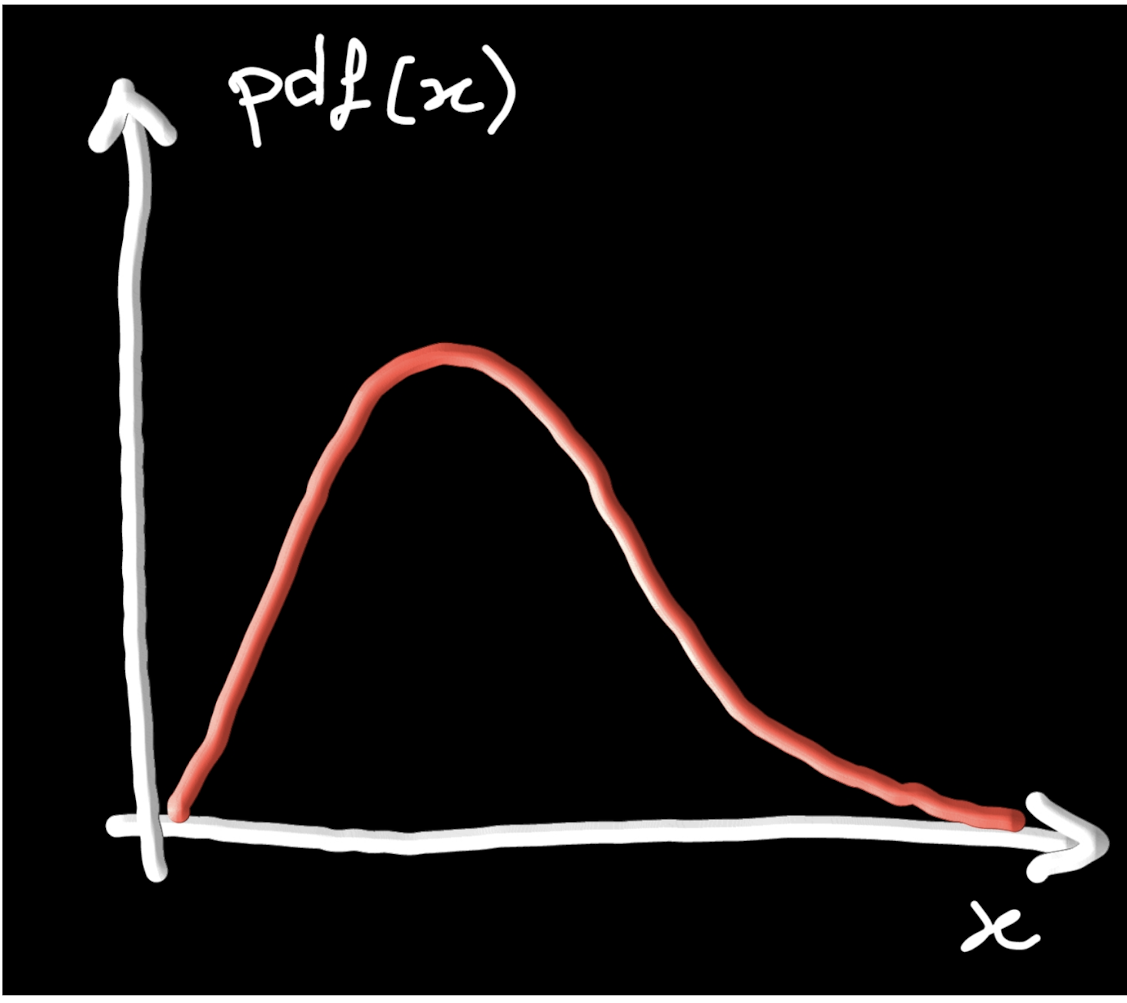
\includegraphics[width=5cm]{pdf} }}
    \qquad
    \subfloat[\centering $P(a<x<b)$]{{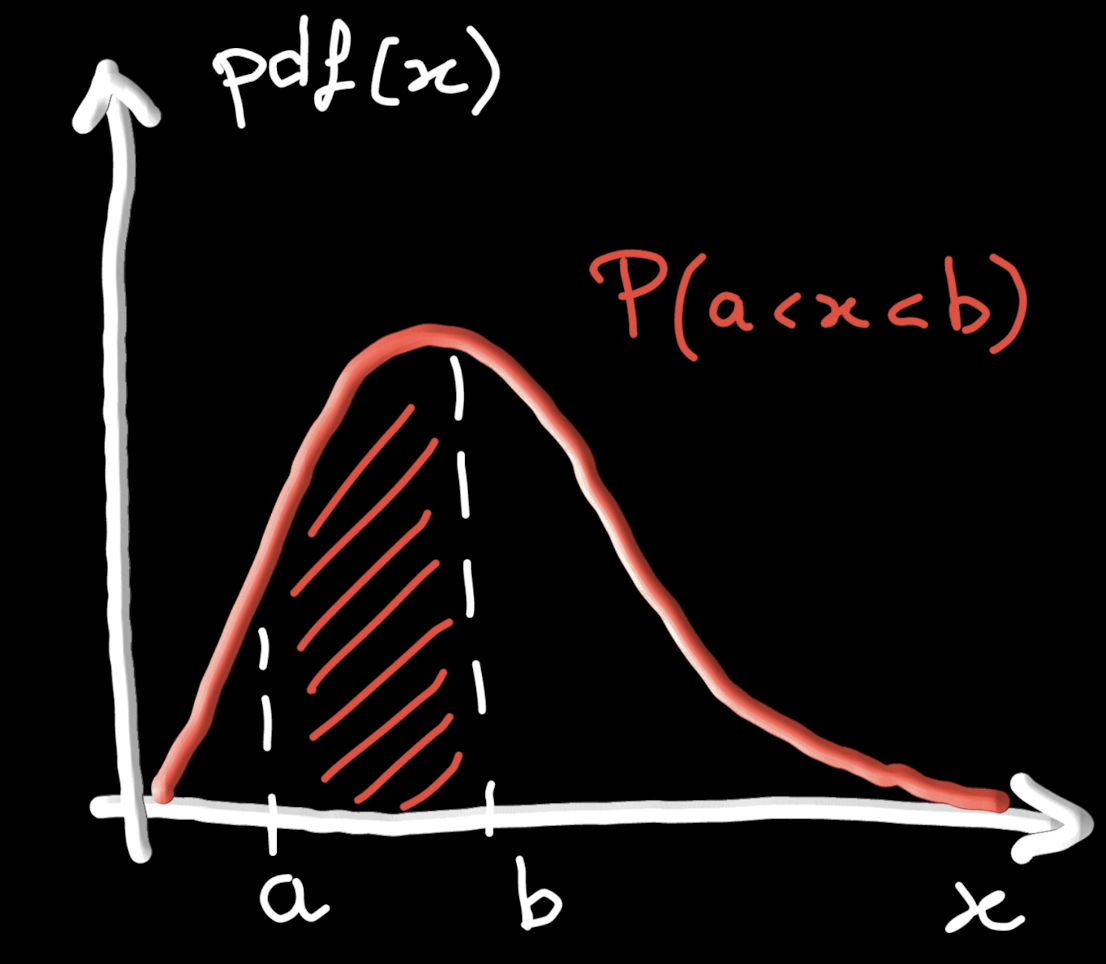
\includegraphics[width=5cm]{prob_pdf} }}
\end{figure}

\subsection{Cumulative distribution function (C.d.f)}

\textcolor{blue}{Che cos\'{e} una c.d.f.?} \newline

Si definisce distribuzione cumulativa la primitiva dell'integrale della pdf di una variabile aleatoria continua \textbf{x}:

\begin{equation}
	cdf(x) = \int_{a}^{x}{pdf(x)dx}
\end{equation}

\noindent ovvero si ha che:

\begin{equation}
	\dfrac{d}{dx}cdf(x)  = pdf(x)
\end{equation}

di conseguenza la cdf(x) descrive l'evolversi della probabilit\'{a} di una variabile casuale.
\subsubsection{Propriet\`{a} di unc cdf}
Una cdf gode delle seguenti propriet\`{a}:
\begin{itemize}
	\item \`{E} una funzione monotona crescente  e definita poisitiva 
	\item cdf(x) $\in [0,1]$
	\item $P(a \leq x \leq b) = cdf(a) - cdf(b)$ 
\end{itemize}
\subsubsection{Corollario}

Esiste una forma analitica della cdf(x) di una r.v. $\iff$ la pdf ammette primitiva. 

\begin{figure}[!ht]
	\vspace{0.2in}
    \centering
    \subfloat[\centering $\int{pdf(x)}$]{{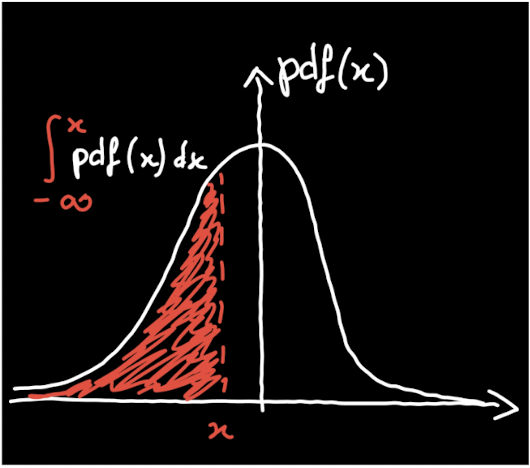
\includegraphics[width=5cm]{int_pdf} }}
    \qquad
    \subfloat[\centering cdf(x)]{{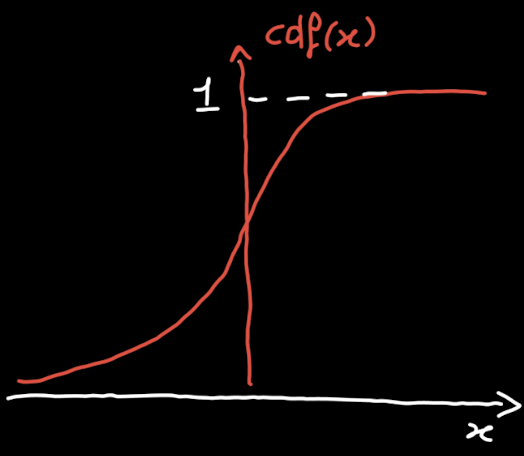
\includegraphics[width=5cm]{cdf} }}
\end{figure}
\newpage
\subsection{Istogrammi}

\textcolor{blue}{Che cos'\'{e} un istogramma ?}\newline


\begin{wrapfigure}{r}{0.\textwidth}
\centering

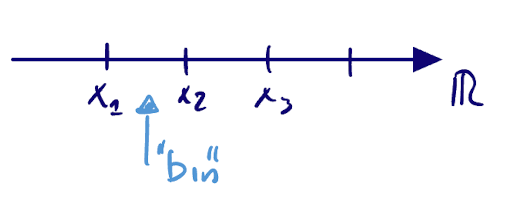
\includegraphics[scale = 0.6]{bin}	

\end{wrapfigure}

Consideriamo una variabile aleatoria x, di cui conosciamo $\{x_i\}_i^N$ valori distinti, utilizziamo tali grandezze come estremi per definire degli intervalli $\omega_{k} = [x_i, x_{i+1}) $ disgiunti tra loro $\omega_{k} \cap \omega_{m} = \varnothing$ per $k \neq m$, sull'asse reale. Tali intervalli vengono definiti \textbf{bin}.

\begin{wrapfigure}[6]{l}{0.\textwidth}

\centering

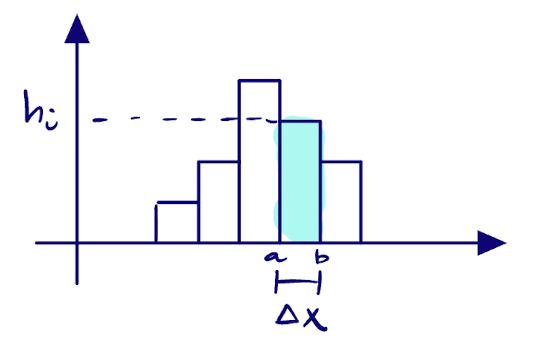
\includegraphics[scale = 0.6]{histogram}	

\end{wrapfigure}

Ripetendo le misure contiamo il numero di volte $n_l$ che un valore compare e cade all'interno di un'intervallo $\omega_k$. 

In questo modo posizionando sull'asse delle ordinate il numero di conteggi $n_l(x)$ si costruisce un istogramma. \newline

\textcolor{blue}{Come si pu\'{o} utilizzare un istogramma per rappresentare una pdf ?}\newline


\begin{wrapfigure}{r}{0.\textwidth}

\centering

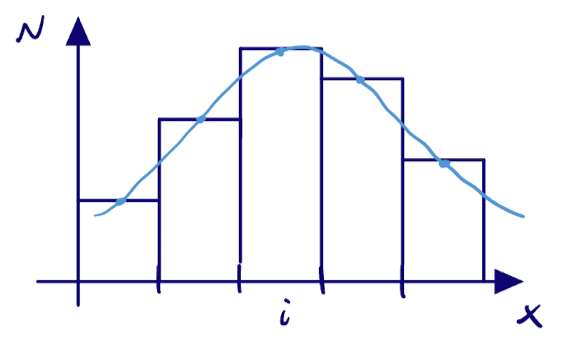
\includegraphics[scale = 0.6]{histo_to_pdf}	

\end{wrapfigure}

All'aumentare del numero di elementi $N \rightarrow \infty$ e diminuendo l'ampiezza dei bin $\Delta x \rightarrow 0 $, ci si riconduce alla nozione di probabilit\'{a} (1.1), in questo modo si passa a una pdf(x) continua.
Per ogni bin \`{e} presente un punto $x_i$ tale che 

\begin{equation*}
	\int_{x_{min}^i}^{x_{max}^i}f(x) dx = f(x_i)\Delta x_i
\end{equation*}
si ha che 
\begin{equation*}
	\lim_{N \rightarrow \infty \atop \Delta \rightarrow 0} \int_{x_{min}^i}^{x_{max}^i}f(x) dx \rightarrow p_i \Rightarrow f(x_i) =  \dfrac{p_i}{\Delta x_i}
\end{equation*}

\subsection{Propriet\`{a} di una probability distribution function}
\textcolor{blue}{Che cosa sono i momenti di una pdf?}\newline

Conoscere l'espressione analitica di una pdf \`{e} spesso poco significativo (soprattuto se la sua espressione non lascia intuire la forma della curva) in altri casi \`{e} impossibile definirla. Di conseguenza per studiare il comportamento di una pdf facciamo affidamento ad alcune grandezze che ne descrivono il comportamento, queste prendono il nome di \textbf{momenti}.

Tali momenti possiamo classificarli come:

\begin{itemize}
	\item $E[x^m] = \int{x^m\cdot pdf(x)dx}$ prendono il nome di \textbf{momenti centrali di ordine m}.
	\item $E[(x-\mu)^m] = \int{(x-\mu)^m \cdot pdf(x)dx}$ prendono il nome di \textbf{momenti centrali}
\end{itemize}

il momento centrale di ordine 1 vale $E[(x-\mu)] = 0$.
\subsection{Valore di aspettazione di una probability distribution function}

\textcolor{blue}{Che cosa \`{e} il valore di aspettazione di una quantit\`{a} rispetto ad una pdf ?}

Data $x \in  \Omega $ variabile aleatoria e $u(x): \mathbb{R} \rightarrow \mathbb{R}$, il valore di aspettazione di u(x) \`{e} definito come:

\begin{equation}
	E[u(x)] = \int{u(x)\cdot pdf(x)dx}
\end{equation}

dove  E[ ] \`{e} un operatore lineare:

\begin{itemize}
	\item $E[x+y] = E[x] + E[y]$
	\item $E[\alpha x] = \alpha E[x] \;\; \forall \alpha \in \mathbb{R}$
\end{itemize}
 Per una variabile aleatoria discreta il valore di aspettazione \`{e} dato da:
 \begin{equation}
 	E[x] = \sum_{i=1}^{+\infty} p_i x_i
 \end{equation}

\subsection{Momenti principali di una pdf per la popolazione e per un campione}

\textcolor{blue}{Che cosa sono e che cosa rappresentano la media, la varianza, l'assimetria e la curtosi di un campione ? e di una popolazione?} \newline

Sia $x \in \Omega $ una variabile aleatoria continua definiamo valore di aspettazione \textbf{media della popolazione} la grandezza:

\begin{equation}
	\mu \equiv E[x] = \int{x \cdot pdf(x)dx}
\end{equation}


\noindent Essa rappresenta il centro della distribuzione di probabilit\`{a} .\newline 
Per un campione di N  misure \textbf{la media} viene definita come: 
\begin{equation}
	\overline{x} = \dfrac{1}{N}\sum_{i=1}^Nx_{i}
\end{equation}
Si definisce \textbf{varianza della popolazione}:
\begin{equation}
	\sigma^2 \equiv V[x] = E[(x-\mu)^2] = \int{(x-\mu)^2 \cdot pdf(x)dx} 	
\end{equation}

la sua radice prende il nome di \textbf{deviazione standard}e definisce l'ampiezza della pdf. La varianza pu\`{o} essere riscritta come:

\begin{equation}
	V[x] = E[x^2] + E[x]^2 = E[x^2] + \mu^2
\end{equation}

Per un campione di N misure \textbf{la varianza} \`{e} data da:

\begin{equation}
	\sigma^2 = \dfrac{1}{N}\sum_{i=1}^N(x- \mu)^2
\end{equation}

mentre \textbf{la deviazione standard} \'{e} di un campione \'{e} data da:

\begin{equation}
	\sigma = \sqrt{\dfrac{1}{N}\sum_{i=1}^N(x- \mu)^2}
\end{equation}

Tra i momenti centrali sono anche presenti la \textbf{skewness} per un campione di N misure:

\begin{equation}
	\gamma_{1} = \dfrac{1}{N}\sum_{i=1}^N \dfrac{(x-\mu)^3}{\sigma^3}
\end{equation}
 e per la popolazione:
 
 \begin{equation}
 	\gamma_{1} = \dfrac{E[(x-\mu)^3]}{\sigma^3}
 \end{equation}
 
 tale grandezza definisce la simmetria di una distribuzione di probabilit\'{a} rispetto al valore centrale dato dal valore di aspettazione $\mu$ per una popolazione. Se una distribuzione \'{e} simmetrica $\gamma_{1} = 0 $.
 
  
\begin{figure}[!ht]

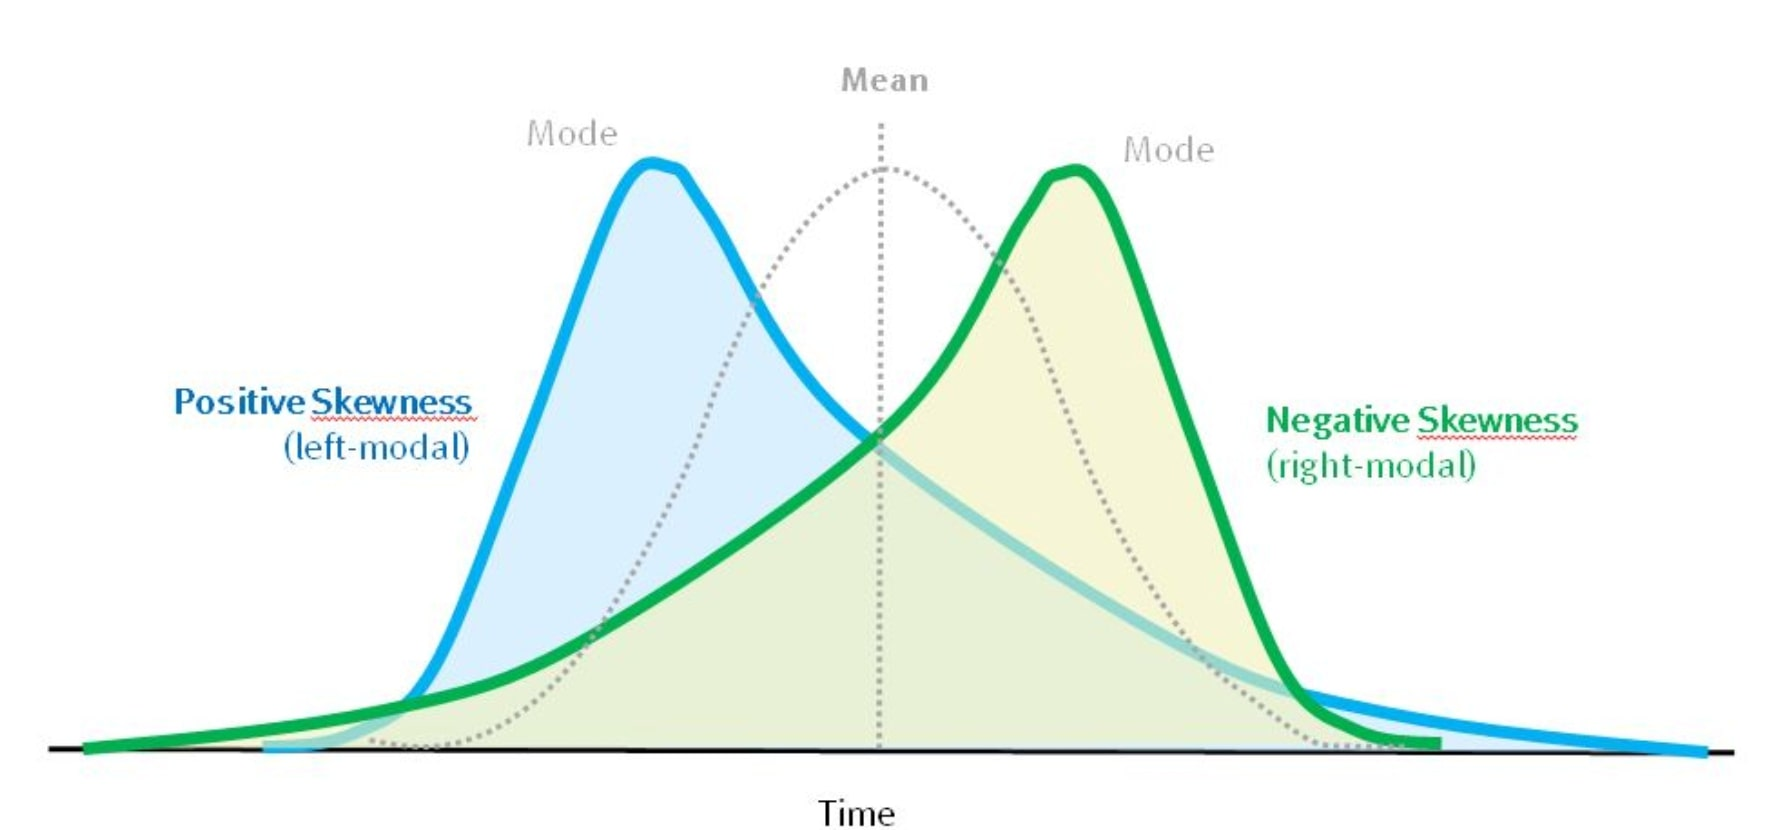
\includegraphics[scale = 0.15]{skew.jpeg}	
\centering
\caption{Simmetria di una distribuzione di probabilit\`{a}}
\end{figure}


Si definisce indice di \textbf{kurtosi} di un campione di N elementi:

\begin{equation}
	\gamma_{2} = \dfrac{1}{N}\sum_{i=1}^N\dfrac{(x-\mu)^4}{\sigma^4}-3
\end{equation}

mentre per la popolazione \`{e} data da:

\begin{equation}
	\gamma_2 = \dfrac{E[(x-\mu)^4]}{\sigma^4} -3
\end{equation}

tale stima fornisce informazioni sul peso delle code della distribuzione, nel senso che per code significative la distribuzione risulter\`{a} pi\`{u} schiacciata nell'intorno del valore $\mu$, mentre per code meno incidenti sar\`{a} pi\'{u} piccata.


\begin{figure}[!ht]

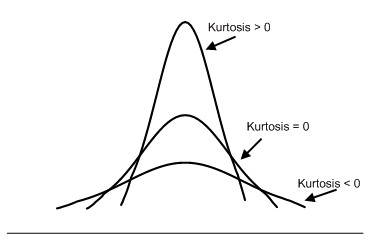
\includegraphics[scale =3.5]{kurtosis.png}	
\centering
\caption{Kurtosi di una distribuzione di probabilit\`{a}}
\end{figure}


\subsubsection{Stime di tendenza centrale}

\textcolor{blue}{Che cosa sono moda, media e mediana di un campione? e di una popolazione ?}


\begin{wrapfigure}[8]{l}{0.\textwidth}

\centering

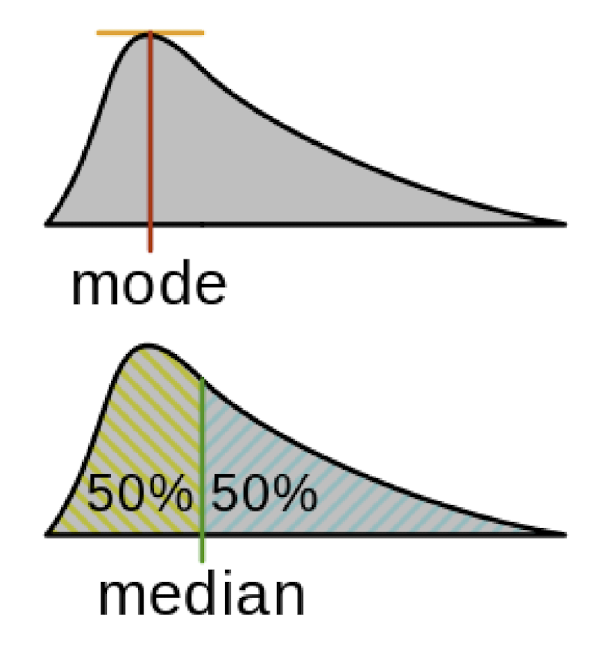
\includegraphics[scale = 0.2]{mod_med}	

\end{wrapfigure}


\noindent Definiamo \textbf{moda} di una popolazione il valore che definisce il massimo della pdf. Mentre per un campione la moda \`{e} definita dalla misura che possiede la frequenza relativa maggiore.\newline

\noindent Mentre si definisce \textbf{mediana} il valore che  divide in due parti uguali la pdf. Nel caso dei campioni le grandezza diventano rispettivamente il valore che compare con maggior frequenza e la misura che divide in due parti eguali il campione.

Per media e mediana di una distribuzione sono unici mentre per una distribuzione pu\`{o} avere pi\`{u} mode, in questi casi si parla di distribuzione \textbf{multimodale}.

 
\begin{figure}[ht]
\vspace{0.3in}
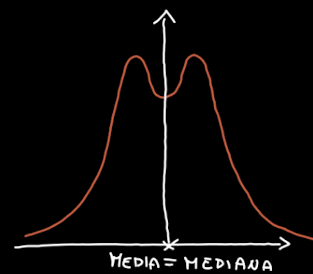
\includegraphics[scale = 0.5]{multimod}	
\centering
\vspace{0.3in}
\caption{Distribuzione multimodale}
\end{figure}

\section{Trasformazioni di distribuzioni di probabilit\`{a}}

Sia x una variabile aleatori continua  che segue una pdf(x) e ipotizziamo di voler costruire una nuova variabile aleatori y legandola ad x mediante una funzione f(x), come definiamo la pdf(y) ?

Sappiamo che la probabilit\`{a} che una misura cada in un intervallo [a,b) \`{e} data da 

\begin{equation*}
	P(a < x< b) = \int_{a}^{b}{pdf(x)dx}
\end{equation*}
\newline

Se effettuiamo un cambio di variabii y=f(x) vogliamo inanzitutto che la trasformazione sia biunivoca dunque f(x) deve essere monotona e continua. In questo modo applicando il teorema per il cambio di coordinate sotto segno d'integrale si ha che:

\begin{equation}
	\dfrac{dy}{dx} = f'(x) \Rightarrow dx = f'(x)^{-1}dy
\end{equation}

di conseguenza:

\begin{equation*}
	P(a < x< b) = \int_{a}^{b}{pdf(x)dx} = \int_{f(a)}^{f(b)}{pdf(y)\vert f'(x)^{-1}\vert dy}
\end{equation*}

per comodit\`{a} si \`{e} posto un modulo affinch\`{e} la funzione sia sempre positiva. In conclusione si ha che:

\begin{equation}
	pdf(y) = pdf(x)\vert f'(x) \vert
\end{equation}
 
 Nel caso in cui abbia pi\`{u} di una dimensione \`{e} necessario che la funzione sia differenziabile e monotona e il modulo della derivata prima della funzione di cambio delle variabili viene sostituita dal modulo del determinante dell'inversa della matrice Jacobiana.
 
 \begin{equation}
 	pdf(\bold{y}) = pdf(\bold{x}) \cdot \vert detJ \vert
 \end{equation}
\newline
\noindent Come si osserva dalle equazioni (1.21) e (1.22) la nuova pdf(y) aumenta o diminuisce di un fattore rispetto alla pdf(x). Comunque sia la probabilit\`{a} in un intervallo resta invariata.

Resta da discutere come cambiano i momenti della distribuzione, per farlo suddividiamo i risultati in due casi:

\subsubsection{Caso in cui il cambio di variabile \`{e} lineare y = ax+b}

Il valore di aspettazione per una pdf(y) dove y = ax+b diventa:

\begin{equation}
	E[y] = \int{y\cdot pdf(y)dy} = \int{(ax+b) \cdot pdf(x)dx = y(\mu_x)}
\end{equation}
 
 analogamente la varianza sar\`{a} data da:
 
 \begin{equation}
 	V[y] = E[y^2] - E[y]^2 = a^2 \cdot V[x]
 \end{equation}

 \subsubsection{Caso in cui il cambio di variabile \'{e} non lineare y = f(x)}
 
 il valore di aspettazione e la varianza di una pdf(y) per y = f(x) non lineare si stima approssimando con il polinomio di Taylor la funzione y(x) in un'intorno di $\mu_x$ al secondo ordine:
 
 \begin{equation*}
 y(x) \approx y(\mu_x) + \dfrac{dy}{dx}\Big\vert_{x = \mu_x}(x-\mu_x) + \dfrac{1}{2}\dfrac{dy^2}{dx^2}\Big\vert_{x = \mu_x}(x-\mu_x)^2
 \end{equation*}
 \newline
 di conseguenza il valore di aspettazione \`{e}:
 
\begin{equation*}
 	E[y] = \int y \cdot pdf(y)dy = y(\mu_x) + \dfrac{dy}{dx}\Big\vert_{x = \mu_x}\int{(x-\mu_x)\cdot pdf(x)dx} + 
 \end{equation*}
 \begin{equation*}
 	+ \dfrac{1}{2}\dfrac{dy^2}{dx^2}\Big\vert_{x = \mu_x} \int{(x-\mu_x)^2 \cdot pdf(x)dx} = 
 \end{equation*}
 
 \begin{equation}
 	= \colorbox{cyan}{\textcolor{white}{$y(\mu_x) + \dfrac{1}{2}\dfrac{dy^2}{dx^2}\Big\vert_{x = \mu_x} \cdot \sigma_{x}^2$}}
 \end{equation}
\newline

Mentre la varianza viene si ottiene dalla relazione:

\begin{equation}
	V[y] = E[y^2] - E[y]^2 = \colorbox{cyan}{\textcolor{white}{$\Big(\dfrac{dy}{dx}\Big \vert_{x = \mu_x}\Big)^2 \cdot \sigma_{x}^2$}} 
\end{equation}
\newline
L'espressione (1.26) \`{e} alla base della formula di propagazione degli errori.

\section{Assenza di memoria per una distribuzione di probabilit\`{a}}

Gli eventi Poissoniani sono indipendenti l'uno dall'altro e la loro probabilit\`{a} di decadimento \`{e} costante, dunque definita q(t) la probabilit\`{a} che non si verifichi un evento in un intervallo di tempo [0,t] si ha che: 
\begin{equation}
	q(t + \delta t) = q(t)q(\Delta t)	
\end{equation}

 la (1.27) definisce l'assenza di memoria di una distribuzione. Si pu\`{o} dimostrare che una distribuzione ha assenza di memoria $\iff$ \`{e} esponenziale.



